\begin{frame}[fragile]{References (1): What are REFS?}
  \begin{itemize}
    \item a reference is a pointer to a commit
    \item git stores these as simple files
  \end{itemize}

\begin{lstlisting}[style=ShellCmd]
$ find .git/refs
.git/refs
.git/refs/heads
.git/refs/tags
$ find .git/refs -type f
\end{lstlisting}
  \begin{itemize}
    \item we can write them manually
  \end{itemize}
\begin{lstlisting}[style=ShellCmd]
$ echo '970ac2c0207ad51caccce0a71d21283ff7109254' \
  > .git/refs/heads/master
$ git log --pretty=oneline master
970ac2c0207ad51caccce0a71d21283ff7109254 third commit
0d9d54e2c438e22d6656fa1bdca7d76a36d3589c second commit
35f8b9255a9c68f80d90201ae14c39d9c9b66b2a first commit
\end{lstlisting}
\end{frame}

\begin{frame}[fragile]{References (2): Branches}
  \begin{itemize}
    \item we can use git update-ref instead
  \end{itemize}

\begin{lstlisting}[style=ShellCmd]
$ git update-ref refs/heads/master \
  970ac2c0207ad51caccce0a71d21283ff7109254
\end{lstlisting}

  \begin{itemize}
    \item each branch is just a simple REF (i. e. a pointer)
    \item we can create one easily
  \end{itemize}
\begin{lstlisting}[style=ShellCmd]
$ git update-ref refs/heads/test \
  0d9d54e2c438e22d6656fa1bdca7d76a36d3589c
$ git log --pretty=oneline test
0d9d54e2c438e22d6656fa1bdca7d76a36d3589c second commit
35f8b9255a9c68f80d90201ae14c39d9c9b66b2a first commit
\end{lstlisting}
\end{frame}

\begin{frame}[fragile]{References (3): Branches continued}
  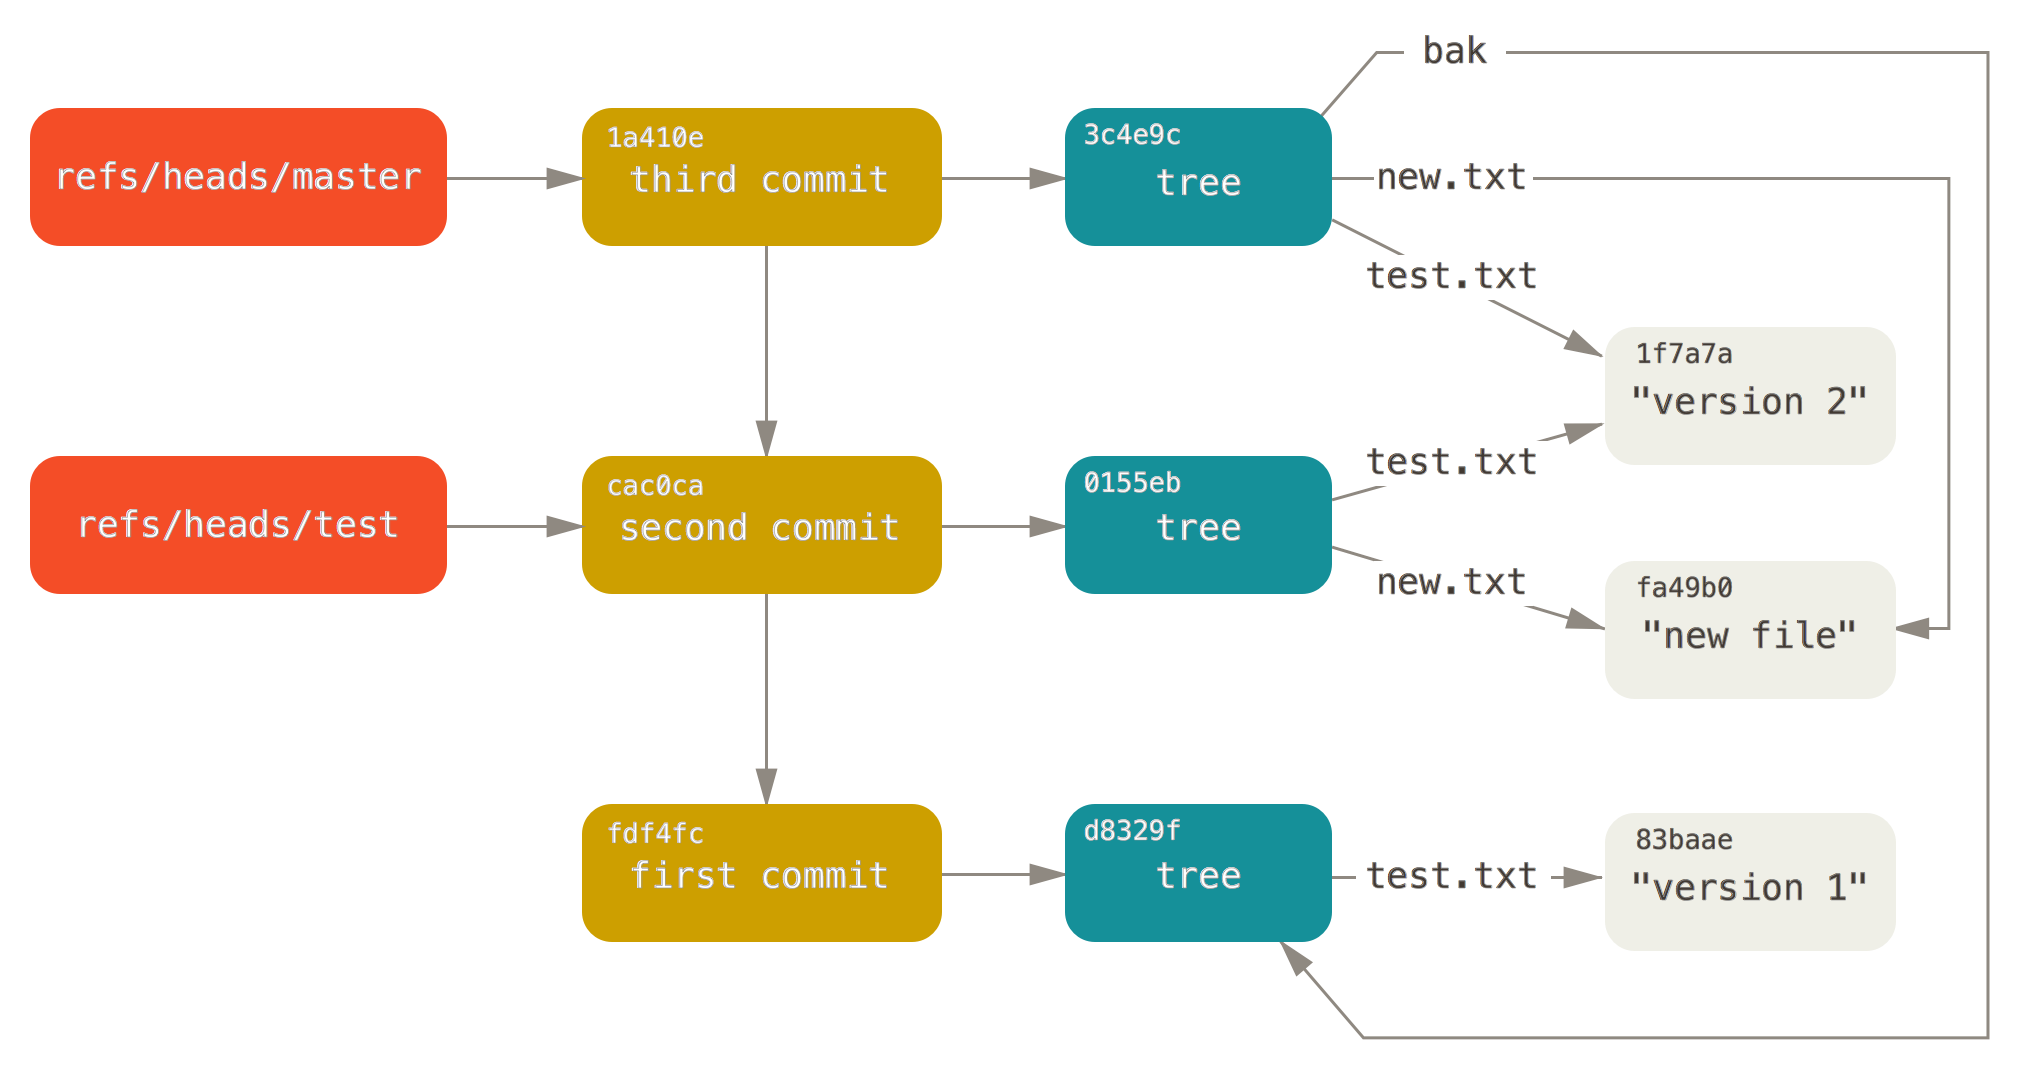
\includegraphics[width=0.90\textwidth]{imgs/branch_tree}
\end{frame}

\begin{frame}[fragile]{References (4): The HEAD}
  \begin{itemize}
    \item the HEAD is a \textit{symbolic} reference to the current branch
    \item each branch has its own HEAD (as you have already seen)
  \end{itemize}
\begin{lstlisting}[style=ShellCmd]
$ cat .git/HEAD
ref: refs/heads/master
$ git checkout test
$ cat .git/HEAD
ref: refs/heads/test
\end{lstlisting}
\begin{itemize}
  \item we could write the symbolic-ref manually
  \item but we can better use
\end{itemize}
\begin{lstlisting}[style=ShellCmd]
$ git symbolic-ref HEAD refs/heads/test
$ cat .git/HEAD
ref: refs/heads/test
\end{lstlisting}
\end{frame}

\begin{frame}[fragile]{References (5): TAGs}
  \begin{itemize}
    \item TAGs are similar to commits
    \item they point to a given version (identified by a commit)
    \item can be light-weight or annotated
    \item we do not go into details here
  \end{itemize}
\end{frame}

\begin{frame}[fragile]{References (6): Remotes}
  \begin{itemize}
    \item remotes are similar to branches
    \item they are considered \textit{read-only}
    \item whenever we fetch / push, they are updated
    \item we will go into remotes in a later section
  \end{itemize}
\end{frame}